\documentclass{beamer}

\usepackage[utf8]{inputenc}
\usetheme{default}

%% set colours
\definecolor{atugreen}{HTML}{005b5e}
\setbeamercolor{title}{fg=atugreen}
\setbeamercolor{frametitle}{fg=atugreen}
\setbeamercolor{section in toc}{fg=atugreen}
\setbeamertemplate{section in toc}{\inserttocsectionnumber.~\inserttocsection}

\title{GLM Model Selection and Validation}
\author{Cóilín Minto, Olga Lyashevska}
\date{July 15\textsuperscript{th} 2022}
\institute{Marine and Freshwater Research Centre\\ Atlantic Technological University \\ Galway, Ireland}
%% logo
\titlegraphic{
    
\includegraphics[width=4cm]{figures/ATU-Logo-Full-RGB-Green-big.jpg}
}

\AtBeginSection[]{
\begin{frame}[noframenumbering, plain]
\frametitle{Outline}
\tableofcontents[currentsection]
\addtocounter{page}{-1}
\end{frame}
}

\begin{document}

\begin{frame}
 \maketitle
\end{frame}

\section{Model Selection}

% \begin{frame}
%  \frametitle{Describe these data}
%  \begin{center}
%     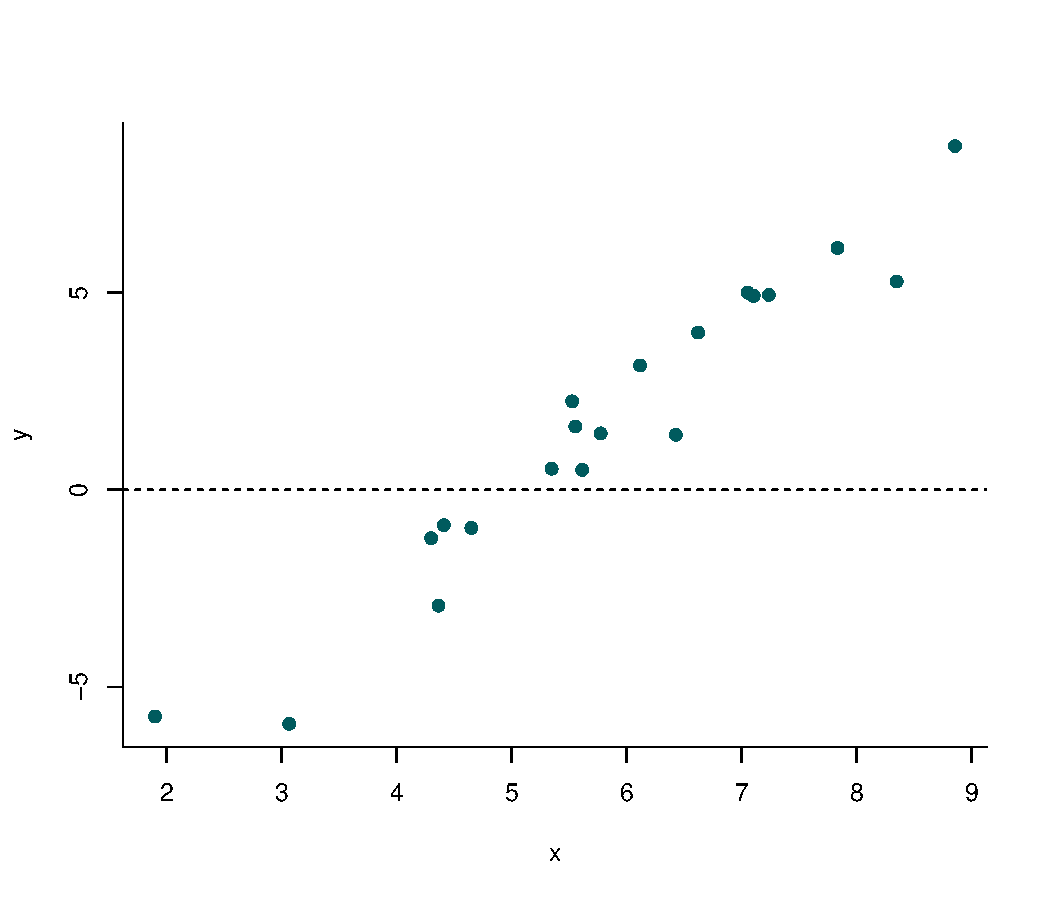
\includegraphics[width=10cm]{figures/continuous_y_0.pdf}
%  \end{center}
% \end{frame}

\begin{frame}{All models are wrong but some are useful}{}

\begin{itemize}
\item Statistical models are mathematical approximations to reality that represent the important features of data for the
task at hand.
\pause
\item The purpose of a statistical model effects how it is developed: prediction versus interpretation
\pause
\item For any set of data, there are numerous components that could be chosen. How
do we choose a statistical model? Statistical models are based on underlying theory, or from an
understanding of the biological features, and are built with
this knowledge in mind. 
\end{itemize}

\end{frame}

\begin{frame}{Criteria}{}
An adequate statistical model balances two criteria:
\begin{itemize}
\item \textbf{Accuracy:} The model should accurately describe both the systematic (fixed) and random components.
\item \textbf{Parsimony:} The model should be as simple as possible. The simplest accurate model is the preferred model. Complex models may fit the given data well but usually do not generalize well to other data sets (over-fitting).
\end{itemize}
\end{frame}


\section{Model Validation}
diagnostics


\section{Assumption Checking}


\section{Principles for improved statistical ecology}

\begin{frame}{Four principles for improved statistical ecology}{ISEC 2022, Session 18. Statistical Theory. Gordana Popovic}

\begin{enumerate}
    \item First define a focused research question, then plan sampling and analysis to answer it; 
    \item Develop a model that accounts for the distribution and characteristics (dependencies) of your data;
    \item Emphasise effect sizes to replace statistical significance (p-values) with ecological relevance;
    \item Report you methods and finding in sufficient detail so that your research is valid and reproducible;
\end{enumerate}
\end{frame}




\end{document}
